\documentclass[a4]{scrartcl}

\usepackage[ngerman]{babel}
\usepackage[utf8]{inputenc}
\usepackage{mathtools}
\usepackage{amsmath}
\usepackage{amssymb}
\usepackage{geometry}
\usepackage{scrpage2}
\pagestyle{scrheadings}
\clearscrheadfoot

\setlength{\parindent}{0em}

\geometry{
  paper=a4paper, % Change to letterpaper for US letter
  top=2cm, % Top margin
  bottom=1.5cm, % Bottom margin
  left=2cm, % Left margin
  right=3cm, % Right margin
  %showframe, % Uncomment to show how the type block is set on the page
}

\ohead{\\
Pina Kolling}


\begin{document}

\subsection*{Vorlesung 3}

\textbf{Digitaler Zwilling}

\begin{itemize}
\item digitale Darstellung eines realen Objekts oder Systems (materiell oder immateriell)
\end{itemize}

\textbf{Integrationsansätze}

\begin{itemize}
\item \textbf{Datenintegration:} Datenbestände von mehreren Informationssystemen werden zentral gespeichert (nicht mehrfach)
\item \textbf{Funktionsintegration:} mehrere Funktionen werden in einem Informationssystem gebündelt
\item \textbf{Prozess- oder Vorgangsintegration:} Prozesse folgender Funktionalitäten sind nahtlos miteinander verbunden (Schnittstellen)
\end{itemize}

\textbf{SAP}
\begin{itemize}
\item Kundenauftrag wird erfasst
\item automatisches Ausführen von: Bestellung der Rohmaterialien, Erzeugung von Fertigungsaufträgen, Übermittlung an die Finanzplanung
\item Rollen \& Rechte verteilen
\end{itemize}

\textbf{ERP Systeme}

$\rightarrow$ integrierte betriebswirtschaftliche Softwarelösungen, die eine Vielzahl Geschäftsprozesse eines Unternehmens abdecken
\begin{itemize}
\item hohe Datenintegration: zentrale Datenbank
\item hohe Funktions- und Prozessintegration: Schnittstellen
\end{itemize}

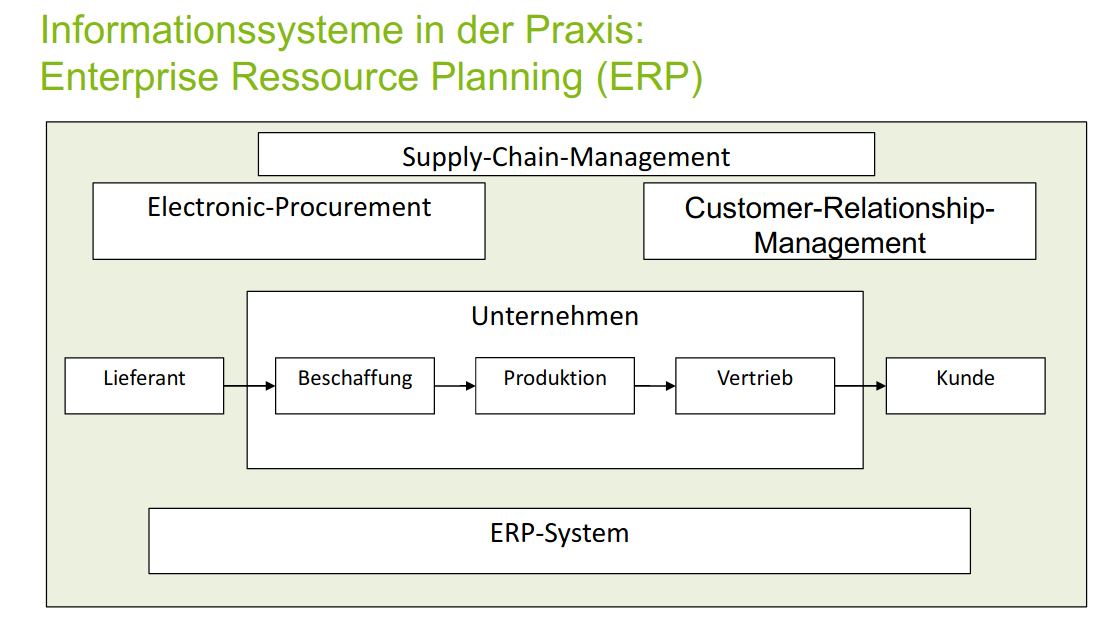
\includegraphics[scale=0.3]{digi_pic.png}

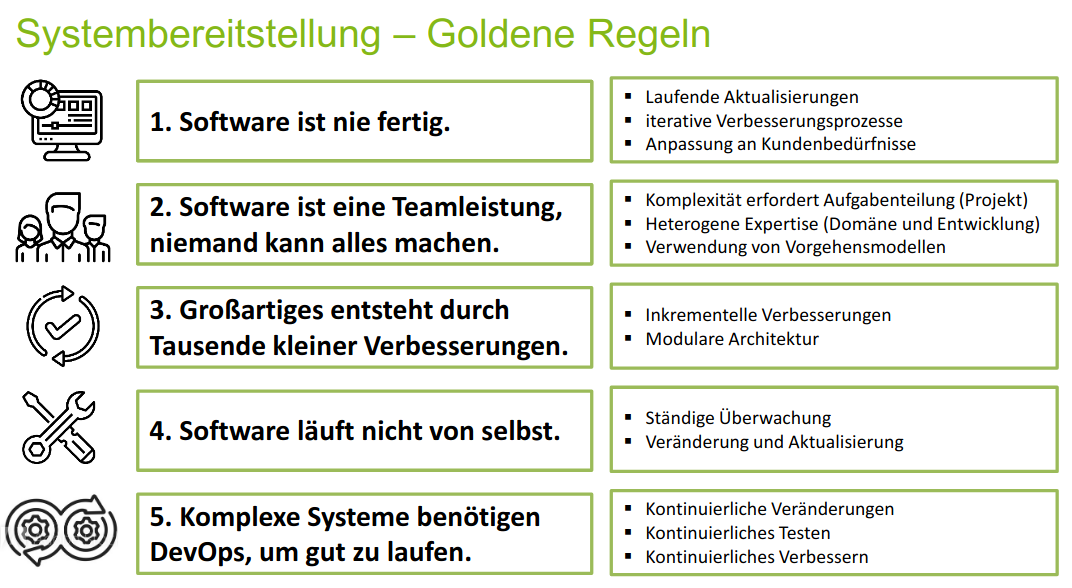
\includegraphics[scale=0.3]{GoldeneRegeln.png}

\newpage
\textbf{Softwareindustrie}

\begin{itemize}
\item Nutzen eines Programms steigt mit Anzahl der Nutzer
\item keine Vervielfältigungskosten: Software kann mehrfach verkauft werden ohne Mehraufwand
\item kein Wertverlust durch Gebrauch
\end{itemize}

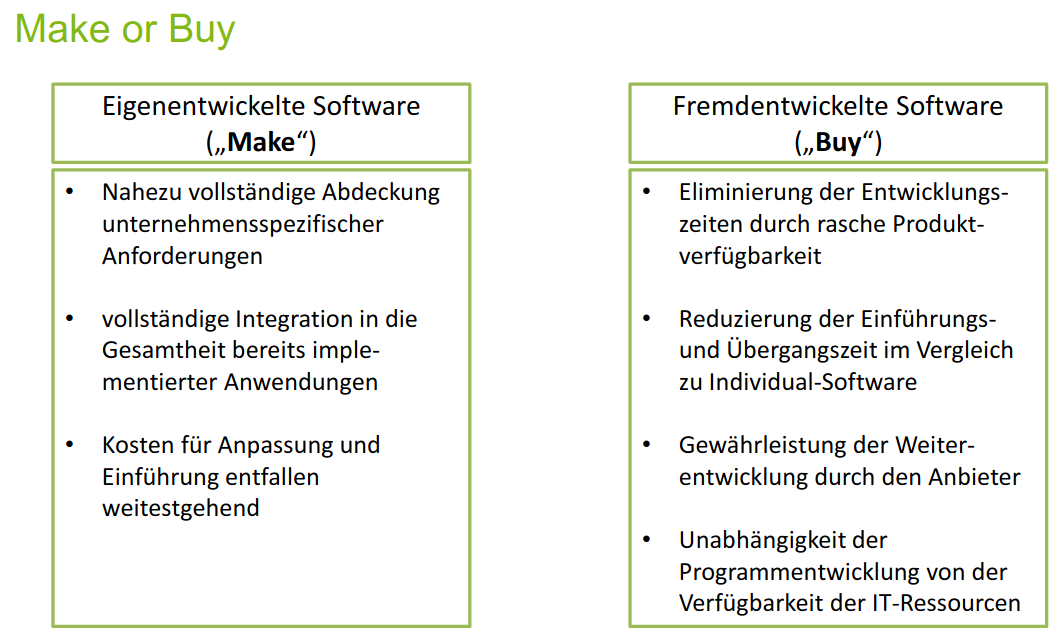
\includegraphics[scale=0.3]{MakeOrBuy.png}

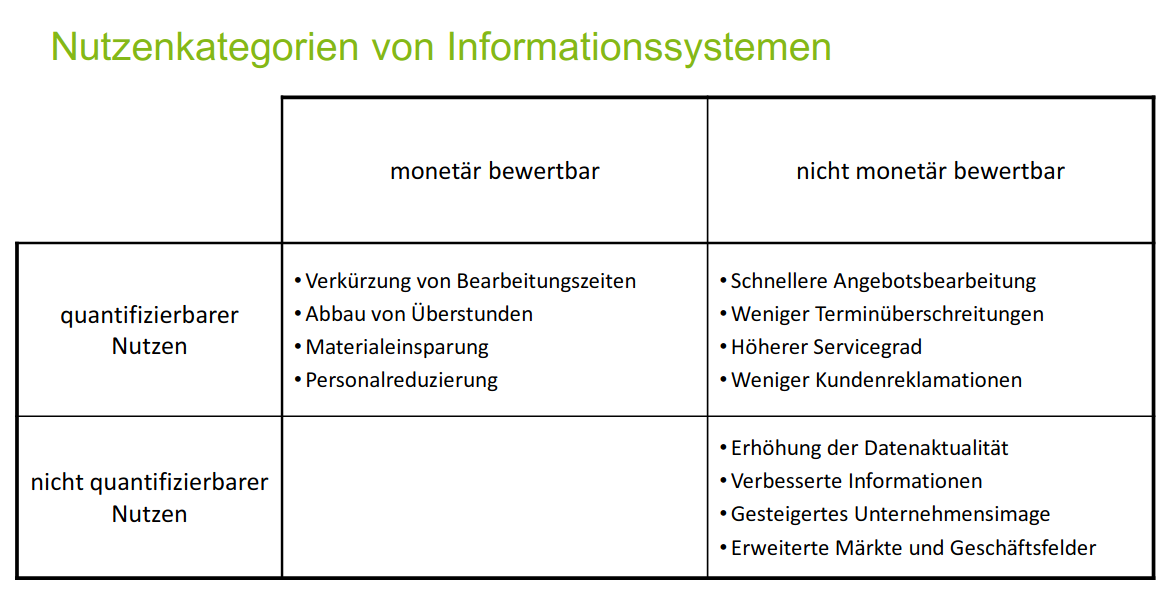
\includegraphics[scale=0.3]{Nutzen.png}

\textbf{Anwendungslebenszyklus}

\begin{itemize}
\item Entwicklung
\item Einführung
\item Wachstum
\item Sättigung/Reife
\item Rückgang
\item Abschaffung
\end{itemize}

\textbf{Planung eines Softwareentwicklungsprozesses}

\begin{itemize}
\item Anforderungsanalyse und Erstellung einer Spezifikation
\item Design
\item Entwicklung
\item Test und Integration
\item Auslieferung des Produkts
\item Wartung und Support
\end{itemize}


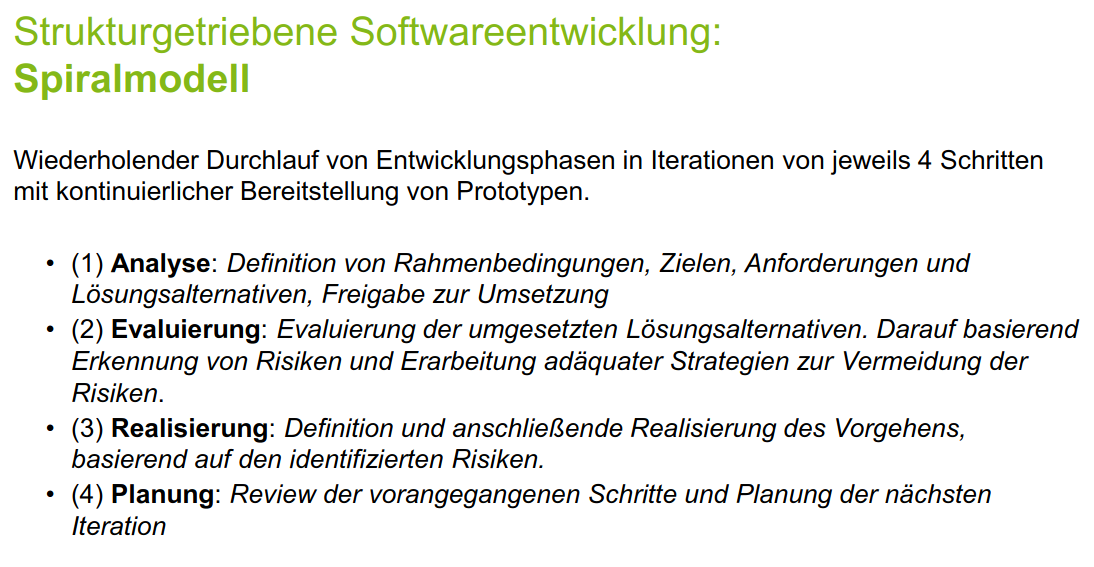
\includegraphics[scale=0.3]{spiralmodell.png}

\textbf{Prinzipien agiler Softwareentwicklung}
\begin{itemize}
\item Transparenz und Geschwindigkeit der Entwicklung erhöhen
\item Fehler minimieren
\item Kommunikation und Interaktion!
\end{itemize}

\textbf{SCRUM}
\begin{itemize}
\item Modell der agilen Softwareentwicklung
\item Transparenz, Überprüfung und Anpassung
\item grober, zeitlicher Rahmen wird definiert und dann angepasst
\item Teams sind selbstorganisiert $\rightarrow$ Daily Meetings
\end{itemize}


\textbf{DevOps}
\begin{itemize}
\item Development + Operations
\item Ziel: in sich veränderden Umgebungen mit schlanken und flexiblen Software-Entwicklungsprozessen schnell zu reagieren
\end{itemize}

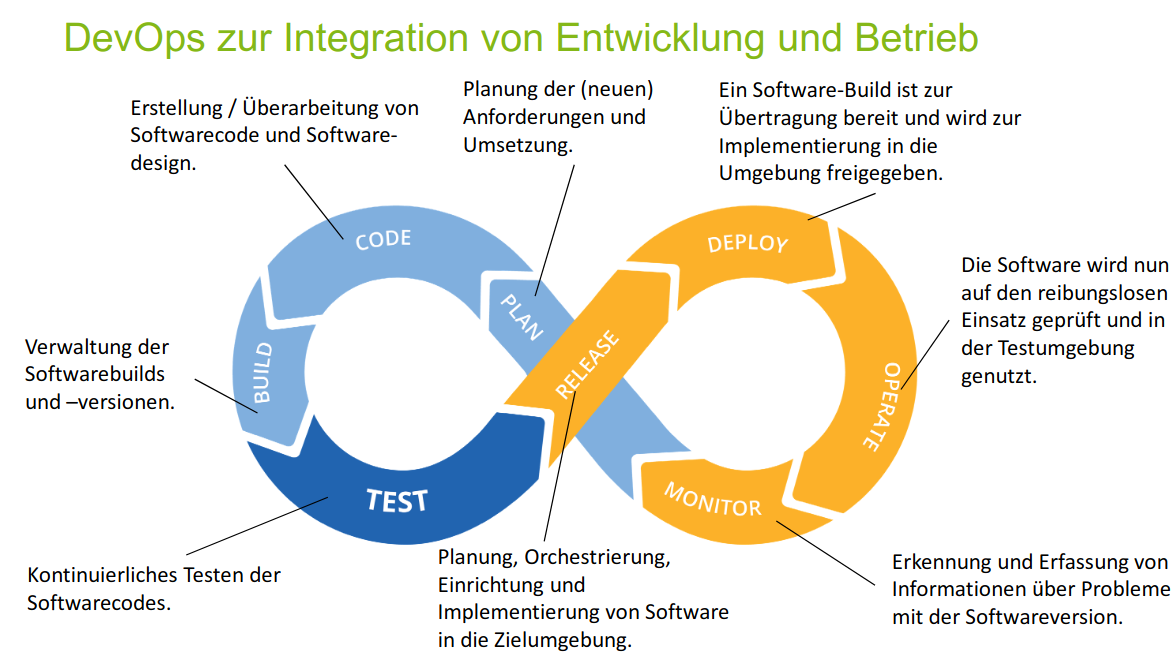
\includegraphics[scale=0.3]{DevOps.png}

\newpage

\textbf{Limitationen und Herausforderungen von DevOps}

\begin{itemize}
\item Flexibilität
\item Automatisierung
\item Lean-Prinzipien $\rightarrow$ System optimieren
\item Alignment-Herausforderung $\rightarrow$ Überwachung der wichtigsten Indikatoren
\item Kultur- und Wissensaustausch
\end{itemize}

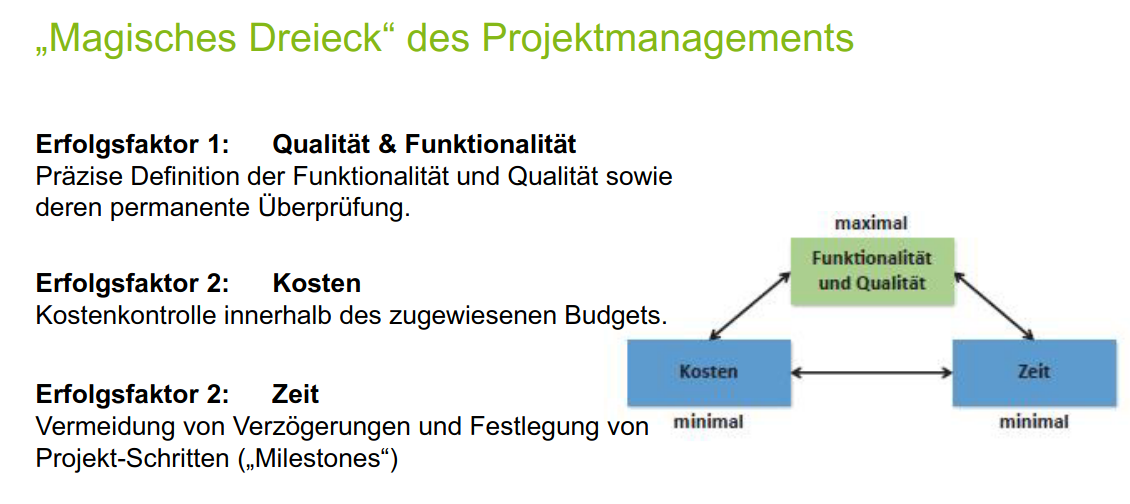
\includegraphics[scale=0.3]{magic.png}

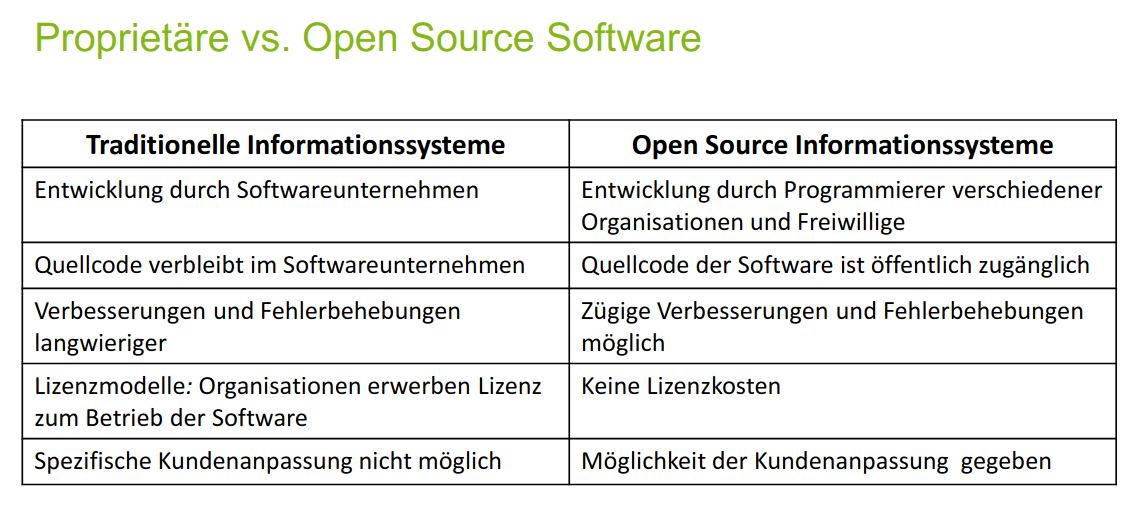
\includegraphics[scale=0.3]{foss.png}



\textbf{Vorgehen zur Softwareauswahl}

\begin{itemize}
\item Ist-Analyse
\item Definition der Anforderung
\item Marktanalyse
\item Vergleich der Angebote
\item Vertragsverhandlung
\end{itemize}



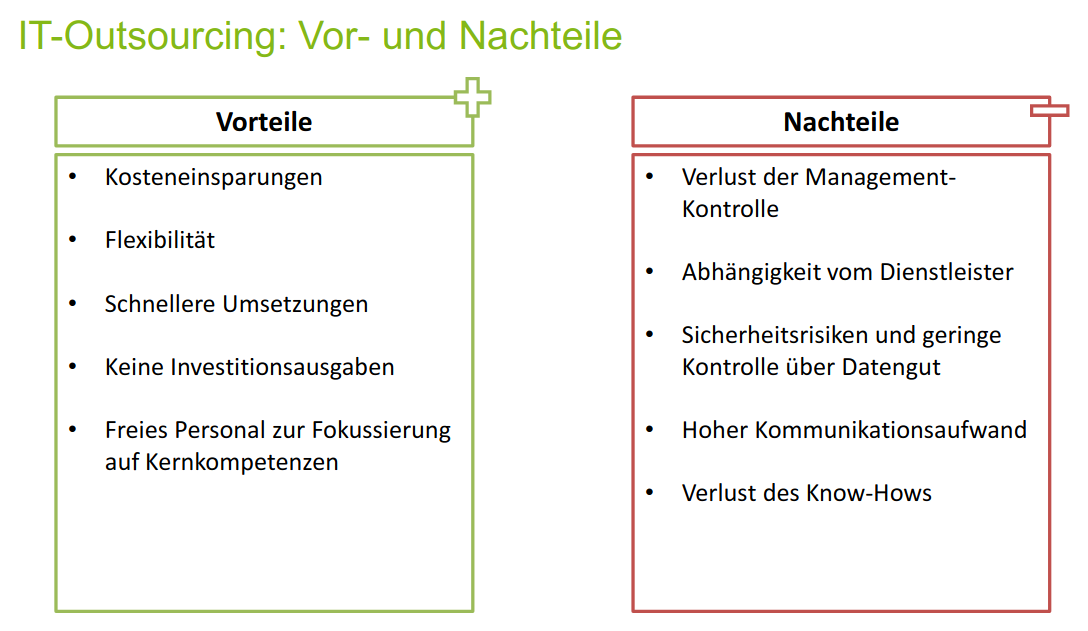
\includegraphics[scale=0.3]{out.png}

















\end{document}






